\documentclass[11pt,a4paper]{article}

% Packages
\usepackage[utf8]{inputenc}
\usepackage[T1]{fontenc}
\usepackage{amsmath,amssymb}
\usepackage{graphicx}
\usepackage{booktabs}
\usepackage{array}
\usepackage{tikz}
\usetikzlibrary{shapes,arrows,positioning,fit,calc,backgrounds,decorations.pathreplacing,arrows.meta}
\usepackage{xcolor}
\usepackage[hidelinks]{hyperref}
\usepackage{geometry}
\geometry{margin=0.9in}
\usepackage{float}
\usepackage{multirow}
\usepackage{enumitem}

% Colors
\definecolor{globalcolor}{RGB}{100, 149, 237}
\definecolor{statecolor}{RGB}{144, 238, 144}
\definecolor{actorcolor}{RGB}{255, 182, 108}
\definecolor{dynamicscolor}{RGB}{255, 160, 160}
\definecolor{ballcolor}{RGB}{221, 160, 221}
\definecolor{querycolor}{RGB}{255, 255, 150}
\definecolor{edgecolor}{RGB}{150, 150, 150}

\title{Cricket Ball Prediction Model V2:\\Unified Heterogeneous Graph Architecture}
\author{Architecture Documentation}
\date{\today}

\begin{document}

\maketitle

\begin{abstract}
This document describes Version 2 of the cricket ball prediction model. The model represents \textbf{all information as a single heterogeneous graph} where different types of nodes (venue, players, match state, ball history) are connected by typed edges that encode cricket-specific relationships. This enables processing full innings history while maintaining computational efficiency through sparse, structured attention patterns.
\end{abstract}

\tableofcontents
\newpage

%==========================================
\section{Overview: What is a Heterogeneous Graph?}
%==========================================

\subsection{The Key Idea}

A \textbf{heterogeneous graph} contains multiple types of nodes and multiple types of edges. Unlike a standard graph where all nodes are the same, our cricket graph has:

\begin{itemize}
    \item \textbf{Different node types}: venue, teams, players, match state, momentum, ball history
    \item \textbf{Different edge types}: ``conditions'', ``matchup'', ``precedes'', ``same\_bowler'', etc.
\end{itemize}

Each edge type can have its own neural network (convolution operator), allowing the model to learn relationship-specific patterns.

\subsection{Why This Matters for Cricket}

Cricket prediction requires understanding many different types of information and their relationships:

\begin{itemize}
    \item \textbf{Who} is batting and bowling (player identities)
    \item \textbf{Where} the match is being played (venue characteristics)
    \item \textbf{What} is the current score, required rate, wickets in hand
    \item \textbf{How} the players are performing today (runs, strike rate, economy)
    \item \textbf{What happened} in previous balls (ball-by-ball history)
\end{itemize}

By encoding all of this in a single graph, the model can learn complex interactions (e.g., ``Rohit struggles against left-arm spin at the MCG in the death overs'').

\newpage
%==========================================
\section{Node Types: The Building Blocks}
%==========================================

The graph contains \textbf{21 context nodes} organized into \textbf{6 categories}, plus N ball history nodes.

\textbf{Important distinction:}
\begin{itemize}
    \item A \textbf{category} is a semantic grouping (e.g., ``Actor'' = all player-related nodes)
    \item Individual \textbf{nodes} within a category represent specific pieces of information
\end{itemize}

\subsection{Category 1: Global (3 nodes)}

These nodes represent match-level constants that don't change during the innings:

\begin{table}[H]
\centering
\begin{tabular}{llp{7cm}}
\toprule
Node Name & Features & What it Represents \\
\midrule
\texttt{venue} & 32-dim embedding & The ground (MCG, Eden Gardens, etc.). Learned embedding captures pitch behavior, boundaries, historical scoring patterns. \\
\texttt{batting\_team} & 32-dim embedding & The team currently batting. Captures team-level tendencies. \\
\texttt{bowling\_team} & 32-dim embedding & The team currently bowling. \\
\bottomrule
\end{tabular}
\caption{Global category: 3 nodes representing match constants}
\end{table}

\textbf{Example:} At the MCG, India batting vs Australia bowling $\to$ venue, batting\_team, bowling\_team nodes initialized with their learned embeddings.

\subsection{Category 2: State (5 nodes)}

These nodes capture the current match situation. They change as the match progresses:

\begin{table}[H]
\centering
\begin{tabular}{llp{6cm}}
\toprule
Node Name & Features & What it Represents \\
\midrule
\texttt{score\_state} & 3 features & Current score, wickets, run rate \\
\texttt{chase\_state} & 3 features & Target, required rate, balls remaining (2nd innings only) \\
\texttt{phase\_state} & 5 features & Powerplay/middle/death phase, over progress, \textbf{is\_first\_ball} indicator \\
\texttt{time\_pressure} & 3 features & Overs remaining, wickets remaining, urgency \\
\texttt{wicket\_buffer} & 2 features & Partnership length, wickets in hand comfort \\
\bottomrule
\end{tabular}
\caption{State category: 5 nodes representing current match situation}
\end{table}

\textbf{Example:} Score 150/3 in 15 overs chasing 180 $\to$ score\_state=(150, 3, 10.0), chase\_state=(180, 6.0, 30), phase\_state=(0, 1, 0, 0.75, 0).

\textbf{Note:} \texttt{is\_first\_ball} in phase\_state is a cold-start indicator (1.0 if this is the very first ball of the innings, 0.0 otherwise).

\subsection{Category 3: Actor (7 nodes)}

These nodes represent the current players on the field and their performance:

\begin{table}[H]
\centering
\begin{tabular}{llp{5.5cm}}
\toprule
Node Name & Features & What it Represents \\
\midrule
\texttt{striker\_identity} & 64-dim embedding & WHO is on strike (learned player embedding) \\
\texttt{striker\_state} & 7 features & HOW they're batting: runs, balls, SR, dot\%, boundaries, set indicator, \textbf{is\_debut\_ball} \\
\texttt{nonstriker\_identity} & 64-dim embedding & WHO is at the non-striker's end \\
\texttt{nonstriker\_state} & 7 features & HOW the non-striker has been batting \\
\texttt{bowler\_identity} & 64-dim embedding & WHO is bowling \\
\texttt{bowler\_state} & 6 features & HOW they're bowling: overs, runs, wickets, economy, dot\% \\
\texttt{partnership} & 4 features & Partnership runs, balls, run rate, boundaries \\
\bottomrule
\end{tabular}
\caption{Actor category: 7 nodes representing current players}
\end{table}

\textbf{Key insight:} Separating identity from state allows the model to learn ``Bumrah is generally accurate'' (identity) independently from ``Bumrah is bowling well today'' (state).

\textbf{Note:} \texttt{is\_debut\_ball} in striker/nonstriker state is 1.0 if this is the player's first ball of the match (cold-start handling).

\subsection{Category 4: Dynamics (4 nodes)}

These nodes capture recent momentum and pressure patterns:

\begin{table}[H]
\centering
\begin{tabular}{llp{6cm}}
\toprule
Node Name & Features & What it Represents \\
\midrule
\texttt{batting\_momentum} & 4 features & Recent scoring rate, boundary\%, acceleration \\
\texttt{bowling\_momentum} & 4 features & Recent economy, dot\%, control \\
\texttt{pressure} & 3 features & Required rate vs actual rate, mounting pressure \\
\texttt{dot\_pressure} & 3 features & Consecutive dots, dot ball spiral indicator \\
\bottomrule
\end{tabular}
\caption{Dynamics category: 4 nodes representing momentum and pressure}
\end{table}

\textbf{Why this matters:} Cricket outcomes are heavily influenced by momentum. A batsman who just hit two boundaries is in a different mental state than one who faced 5 dots.

\subsection{Category 5: Ball (N nodes)}

Each historical ball in the innings becomes a node:

\begin{table}[H]
\centering
\begin{tabular}{lp{9cm}}
\toprule
Features & Description \\
\midrule
15 numeric features & runs, is\_wicket, over, ball\_in\_over, is\_boundary, extras (wide, noball, bye, legbye), wicket types (bowled, caught, lbw, run\_out, stumped, other) \\
64-dim bowler ID & Embedding of who bowled this ball \\
64-dim batsman ID & Embedding of who faced this ball \\
\bottomrule
\end{tabular}
\caption{Ball nodes: one per historical delivery}
\end{table}

\textbf{Total per ball:} 15 + 64 + 64 = 143 features $\to$ projected to 128-dim.

\subsection{Category 6: Query (1 node)}

A special node used to aggregate all information for the final prediction:

\begin{itemize}
    \item Initialized with zeros
    \item After message passing, contains aggregated information from the entire graph
    \item Final prediction is made from this node's representation
\end{itemize}

\subsection{Summary: Total Node Count}

\begin{table}[H]
\centering
\begin{tabular}{lcc}
\toprule
Category & Nodes in Category & Role \\
\midrule
Global & 3 & Match constants \\
State & 5 & Current situation \\
Actor & 7 & Players on field \\
Dynamics & 4 & Momentum/pressure \\
Ball & N (variable) & Full innings history \\
Query & 1 & Prediction aggregation \\
\midrule
\textbf{Total} & \textbf{20 + N} & \\
\bottomrule
\end{tabular}
\caption{Node count by category}
\end{table}

\newpage
%==========================================
\section{Edge Types: The Relationships}
%==========================================

Edges encode \textbf{how nodes relate to each other}. Different edge types have different meanings and use different neural network operations.

\subsection{Understanding Edge Type Notation}

An edge type is written as: \texttt{(source\_type, relation, target\_type)}

For example: \texttt{(global, conditions, state)} means ``global nodes have a 'conditions' relationship with state nodes''.

\textbf{Important:} The categories (global, state, etc.) contain multiple nodes. An edge type like \texttt{(global, conditions, state)} means edges connect nodes \textit{within} those categories.

\subsection{Category 1: Hierarchical Edges (3 types)}

These edges encode a \textbf{top-down conditioning} structure: higher-level context influences lower-level interpretation.

\begin{table}[H]
\centering
\begin{tabular}{llp{5cm}}
\toprule
Edge Type & Connectivity & Meaning \\
\midrule
\texttt{(global, conditions, state)} & 3 $\to$ 5 (15 edges) & Venue/teams influence how we interpret the score \\
\texttt{(state, conditions, actor)} & 5 $\to$ 7 (35 edges) & Match situation influences how we interpret player performance \\
\texttt{(actor, conditions, dynamics)} & 7 $\to$ 4 (28 edges) & Current players influence how we interpret momentum \\
\bottomrule
\end{tabular}
\caption{Hierarchical edges: top-down conditioning}
\end{table}

\textbf{Concrete example:} 150/3 means different things at the MCG (good) vs Chennai (average). The edge from \texttt{venue} to \texttt{score\_state} allows this contextual interpretation.

\subsection{Category 2: Intra-Layer Edges (4 types)}

These edges connect nodes \textbf{within the same category}, allowing related information to interact.

\subsubsection{What does ``global $\leftrightarrow$ global'' mean?}

This means edges between the 3 nodes in the global category:

\begin{figure}[H]
\centering
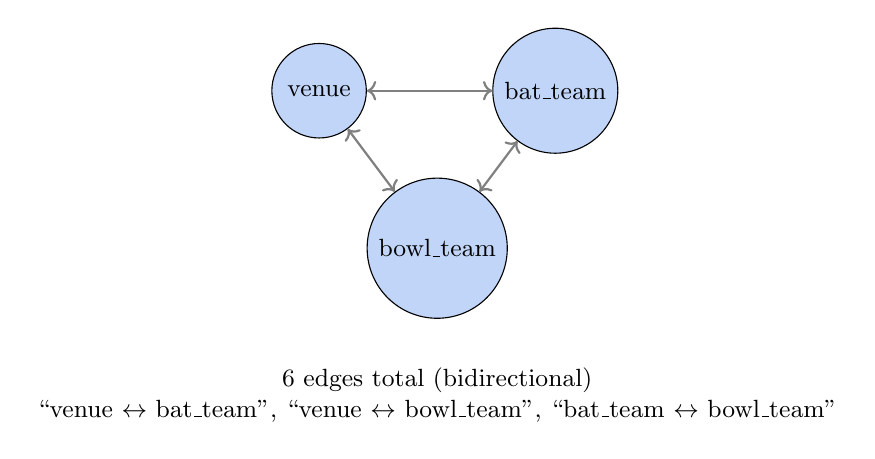
\begin{tikzpicture}[
    node/.style={circle, draw, fill=globalcolor!40, minimum size=1.2cm, font=\small},
    edge/.style={<->, thick, gray}
]
    \node[node] (v) at (0, 0) {venue};
    \node[node] (bt) at (3, 0) {bat\_team};
    \node[node] (bot) at (1.5, -2) {bowl\_team};

    \draw[edge] (v) -- node[above] {} (bt);
    \draw[edge] (v) -- node[left] {} (bot);
    \draw[edge] (bt) -- node[right] {} (bot);

    \node[below=0.5cm of bot, align=center, font=\small] {
        6 edges total (bidirectional)\\
        ``venue $\leftrightarrow$ bat\_team'', ``venue $\leftrightarrow$ bowl\_team'', ``bat\_team $\leftrightarrow$ bowl\_team''
    };
\end{tikzpicture}
\caption{Intra-layer edges within the Global category}
\end{figure}

\textbf{Why it matters:} India playing at home vs Australia playing away is different from the reverse. The venue-team combination matters.

\begin{table}[H]
\centering
\begin{tabular}{llp{4.5cm}}
\toprule
Edge Type & Edges & What it Captures \\
\midrule
\texttt{(global, relates\_to, global)} & 6 & Home/away advantage, venue-team combinations \\
\texttt{(state, relates\_to, state)} & 20 & Score relates to required rate, phase relates to pressure \\
\texttt{(actor, matchup, actor)} & 22 & Striker-bowler confrontation, partnership dynamics \\
\texttt{(dynamics, relates\_to, dynamics)} & 12 & Batting momentum vs bowling momentum (zero-sum) \\
\bottomrule
\end{tabular}
\caption{Intra-layer edges: within-category relationships}
\end{table}

\subsubsection{The Actor Matchup Graph}

The \texttt{(actor, matchup, actor)} edges deserve special attention. They encode:

\begin{figure}[H]
\centering
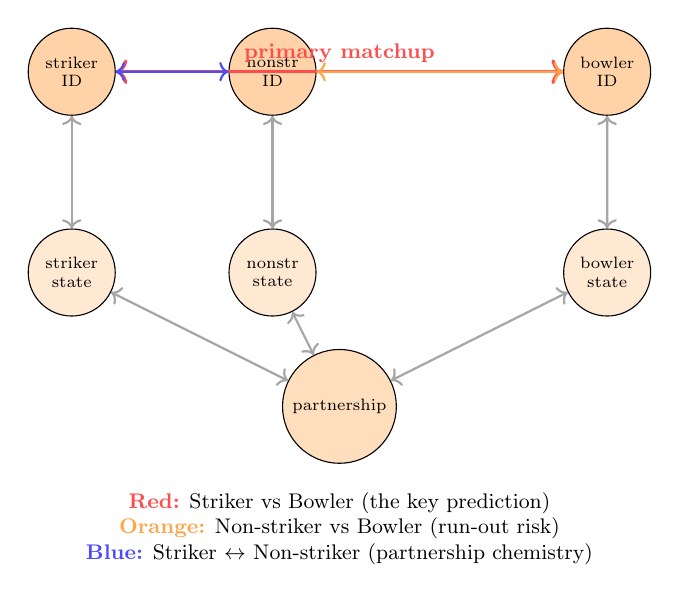
\begin{tikzpicture}[
    identity/.style={circle, draw, fill=actorcolor!60, minimum size=1.3cm, align=center, font=\scriptsize},
    state/.style={circle, draw, fill=actorcolor!30, minimum size=1.3cm, align=center, font=\scriptsize},
    partnership/.style={circle, draw, fill=actorcolor!45, minimum size=1.3cm, align=center, font=\scriptsize},
    edge/.style={<->, thick, gray!70},
    keyedge/.style={<->, very thick, red!70},
    scale=0.85, transform shape
]
    % Striker
    \node[identity] (si) at (-4, 2) {striker\\ID};
    \node[state] (ss) at (-4, -1) {striker\\state};

    % Non-striker
    \node[identity] (ni) at (-1, 2) {nonstr\\ID};
    \node[state] (ns) at (-1, -1) {nonstr\\state};

    % Bowler
    \node[identity] (bi) at (4, 2) {bowler\\ID};
    \node[state] (bs) at (4, -1) {bowler\\state};

    % Partnership
    \node[partnership] (p) at (0, -3) {partnership};

    % Identity <-> State
    \draw[edge] (si) -- (ss);
    \draw[edge] (ni) -- (ns);
    \draw[edge] (bi) -- (bs);

    % Partnership connections
    \draw[edge] (ss) -- (p);
    \draw[edge] (ns) -- (p);
    \draw[edge] (bs) -- (p);

    % THE KEY MATCHUPS
    \draw[keyedge] (si) -- node[above, font=\small] {\textbf{primary matchup}} (bi);
    \draw[edge, orange!70, thick] (ni) -- (bi);
    \draw[edge, blue!70, thick] (si) -- (ni);

    \node[below=0.3cm of p, align=center, font=\small] {
        \textcolor{red!70}{\textbf{Red:}} Striker vs Bowler (the key prediction)\\
        \textcolor{orange!70}{\textbf{Orange:}} Non-striker vs Bowler (run-out risk)\\
        \textcolor{blue!70}{\textbf{Blue:}} Striker $\leftrightarrow$ Non-striker (partnership chemistry)
    };
\end{tikzpicture}
\caption{Actor matchup edges capture player interactions}
\end{figure}

\subsection{Category 3: Temporal Edges (6 types)}

These edges encode the \textbf{structure of ball-by-ball history}. This is where V2 gains efficiency over transformer attention.

\subsubsection{Multi-Scale Temporal Architecture}

Cricket patterns occur at different time scales:
\begin{itemize}
    \item \textbf{Within-over (1-6 balls):} Immediate pressure, bowler's current plan
    \item \textbf{2-over window (7-18 balls):} Momentum shifts, scoring patterns
    \item \textbf{Historical (19+ balls):} Phase patterns, earlier wickets' impact
\end{itemize}

We use \textbf{three separate edge types} for these scales:

\begin{table}[H]
\centering
\begin{tabular}{lp{4cm}p{5cm}}
\toprule
Edge Type & Connects & Neural Network \\
\midrule
\texttt{recent\_precedes} & Balls within 6 deliveries & TransformerConv (fast decay, attention to recency) \\
\texttt{medium\_precedes} & Balls 7-18 apart & TransformerConv (medium decay) \\
\texttt{distant\_precedes} & Balls 19+ apart (sparse) & SAGEConv (simple mean, sparse connections) \\
\bottomrule
\end{tabular}
\caption{Multi-scale temporal edges}
\end{table}

\begin{figure}[H]
\centering
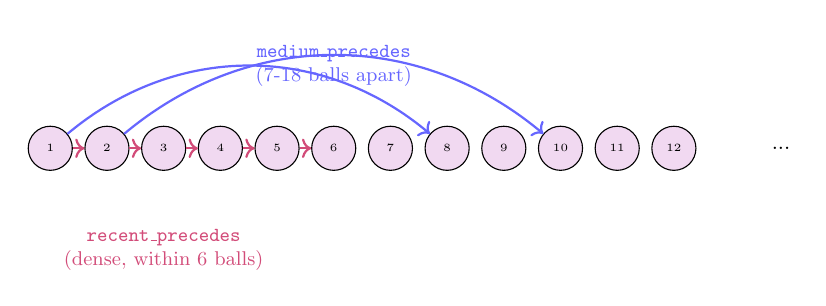
\begin{tikzpicture}[
    ball/.style={circle, draw, fill=ballcolor!40, minimum size=0.7cm, font=\tiny},
    scale=0.8, transform shape
]
    % Balls
    \foreach \i in {1,...,12} {
        \node[ball] (b\i) at (\i*0.9, 0) {\i};
    }
    \node at (12.5, 0) {...};

    % Recent (purple) - dense
    \draw[->, purple!70, thick] (b1) -- (b2);
    \draw[->, purple!70, thick] (b2) -- (b3);
    \draw[->, purple!70, thick] (b3) -- (b4);
    \draw[->, purple!70, thick] (b4) -- (b5);
    \draw[->, purple!70, thick] (b5) -- (b6);

    % Medium (blue) - from ball 1 to 7-12
    \draw[->, blue!60, thick, bend left=40] (b1) to (b8);
    \draw[->, blue!60, thick, bend left=40] (b2) to (b10);

    % Labels
    \node[below=0.8cm of b3, align=center, font=\small, purple!70] {\texttt{recent\_precedes}\\(dense, within 6 balls)};
    \node[above=0.5cm of b6, align=center, font=\small, blue!60] {\texttt{medium\_precedes}\\(7-18 balls apart)};
\end{tikzpicture}
\caption{Multi-scale temporal edges (distant not shown for clarity)}
\end{figure}

\subsubsection{Same-Bowler and Same-Batsman Edges}

These edges connect balls by the same player, regardless of temporal distance:

\begin{figure}[H]
\centering
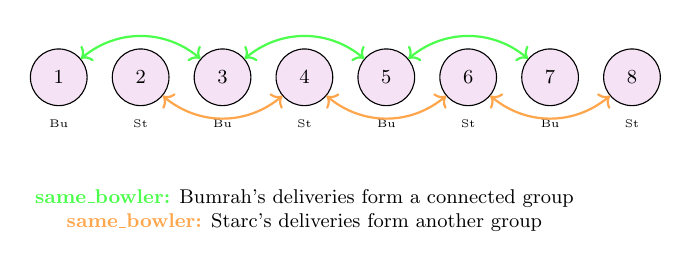
\begin{tikzpicture}[
    ball/.style={circle, draw, minimum size=0.9cm, font=\small},
    scale=0.8, transform shape
]
    % Balls with bowler labels
    \foreach \i/\b in {1/Bu, 2/St, 3/Bu, 4/St, 5/Bu, 6/St, 7/Bu, 8/St} {
        \node[ball, fill=ballcolor!30] (b\i) at (\i*1.3, 0) {\i};
        \node[below=0.1cm of b\i, font=\tiny] {\b};
    }

    % Same bowler: Bumrah (1,3,5,7) - green
    \draw[<->, green!70, thick, bend left=40] (b1) to (b3);
    \draw[<->, green!70, thick, bend left=40] (b3) to (b5);
    \draw[<->, green!70, thick, bend left=40] (b5) to (b7);

    % Same bowler: Starc (2,4,6,8) - orange
    \draw[<->, orange!70, thick, bend right=40] (b2) to (b4);
    \draw[<->, orange!70, thick, bend right=40] (b4) to (b6);
    \draw[<->, orange!70, thick, bend right=40] (b6) to (b8);

    \node[below=1.2cm of b4, align=center, font=\small] {
        \textcolor{green!70}{\textbf{same\_bowler:}} Bumrah's deliveries form a connected group\\
        \textcolor{orange!70}{\textbf{same\_bowler:}} Starc's deliveries form another group
    };
\end{tikzpicture}
\caption{same\_bowler edges group a bowler's spell}
\end{figure}

\textbf{Why this matters:} The model can ask ``How has Bumrah been bowling?'' by looking at all his deliveries together, without needing to attend to balls by other bowlers.

\subsubsection{Same-Matchup Edges (CAUSAL)}

\texttt{same\_matchup} connects balls with the same bowler-batsman combination:

\textbf{Critical:} Unlike same\_bowler/same\_batsman (bidirectional), same\_matchup edges are \textbf{UNIDIRECTIONAL (older $\to$ newer)}. This prevents ``future information leakage'':

\begin{itemize}
    \item During training, the graph contains future balls
    \item Bidirectional edges would let the model ``see'' future outcomes
    \item At inference time, only historical balls exist
    \item Causal edges ensure the model learns patterns valid at inference
\end{itemize}

\begin{figure}[H]
\centering
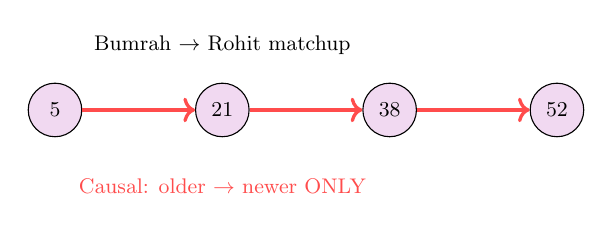
\begin{tikzpicture}[
    ball/.style={circle, draw, fill=ballcolor!40, minimum size=0.8cm, font=\small},
    scale=0.85, transform shape
]
    \node[ball] (b5) at (0, 0) {5};
    \node[ball] (b21) at (2.5, 0) {21};
    \node[ball] (b38) at (5, 0) {38};
    \node[ball] (b52) at (7.5, 0) {52};

    \draw[->, red!70, very thick] (b5) -- (b21);
    \draw[->, red!70, very thick] (b21) -- (b38);
    \draw[->, red!70, very thick] (b38) -- (b52);

    \node[above=0.3cm of b21, font=\small] {Bumrah $\to$ Rohit matchup};
    \node[below=0.5cm of b21, font=\small, red!70] {Causal: older $\to$ newer ONLY};
\end{tikzpicture}
\caption{same\_matchup edges are causal to prevent distribution shift}
\end{figure}

\subsection{Category 4: Cross-Domain Edges (4 types)}

These edges connect ball history to current context nodes:

\begin{table}[H]
\centering
\begin{tabular}{lp{6cm}l}
\toprule
Edge Type & Meaning & Connectivity \\
\midrule
\texttt{(ball, faced\_by, striker\_identity)} & Balls faced by current striker & Variable \\
\texttt{(ball, bowled\_by, bowler\_identity)} & Balls bowled by current bowler & Variable \\
\texttt{(ball, partnered\_by, nonstriker\_identity)} & Balls involving current non-striker & Variable \\
\texttt{(ball, informs, dynamics)} & Recent balls inform momentum & 12 $\to$ 4 \\
\bottomrule
\end{tabular}
\caption{Cross-domain edges connect history to context}
\end{table}

\textbf{Critical: Correct Player Attribution}

Cross-domain edges ONLY connect to balls involving the CURRENT players:

\begin{itemize}
    \item If Kohli faced balls 1-20 then got out, and Sharma is now batting
    \item Balls 1-20 do NOT connect to \texttt{striker\_identity} (which is now Sharma)
    \item Only balls Sharma actually faced will connect
\end{itemize}

This respects the Z2 symmetry of striker/non-striker swapping.

\subsection{Category 5: Query Edges (2 types)}

\subsubsection{Attends Edges}

The query node receives information from all other nodes:

\begin{table}[H]
\centering
\begin{tabular}{ll}
\toprule
Edge Type & Connectivity \\
\midrule
\texttt{(*, attends, query)} & All 20 context nodes + N balls $\to$ query \\
\bottomrule
\end{tabular}
\end{table}

\subsubsection{Drives Edges (NEW)}

Dynamics nodes \textbf{directly drive} prediction through feedback loops:

\begin{table}[H]
\centering
\begin{tabular}{lp{7cm}}
\toprule
Edge Type & Meaning \\
\midrule
\texttt{(dynamics, drives, query)} & Momentum and pressure directly influence prediction \\
\bottomrule
\end{tabular}
\end{table}

\textbf{Why a separate edge type?}

The \texttt{drives} edges capture \textbf{causal feedback loops}:

\begin{enumerate}
    \item \textbf{Confidence Spiral:} High batting momentum $\to$ more aggressive shots $\to$ more runs $\to$ higher momentum
    \item \textbf{Required Rate Pressure:} High pressure $\to$ risk-taking $\to$ boundaries OR wickets
    \item \textbf{Dot Ball Spiral:} High dot pressure $\to$ desperate shots $\to$ wickets $\to$ rebuilding
\end{enumerate}

By having learned attention weights on \texttt{drives} edges, the model can weight different dynamics signals appropriately.

\subsection{Edge Type Summary}

\begin{table}[H]
\centering
\begin{tabular}{lcc}
\toprule
Category & Edge Types & Purpose \\
\midrule
Hierarchical & 3 & Top-down context conditioning \\
Intra-layer & 4 & Within-category interactions \\
Temporal & 6 & Ball history structure (multi-scale + actor grouping) \\
Cross-domain & 4 & Connect history to context \\
Query & 2 & Prediction aggregation + dynamics drive \\
\midrule
\textbf{Total} & \textbf{19} & \\
\bottomrule
\end{tabular}
\caption{19 edge types organized by purpose}
\end{table}

\newpage
%==========================================
\section{Full Graph Visualization}
%==========================================

\begin{figure}[H]
\centering
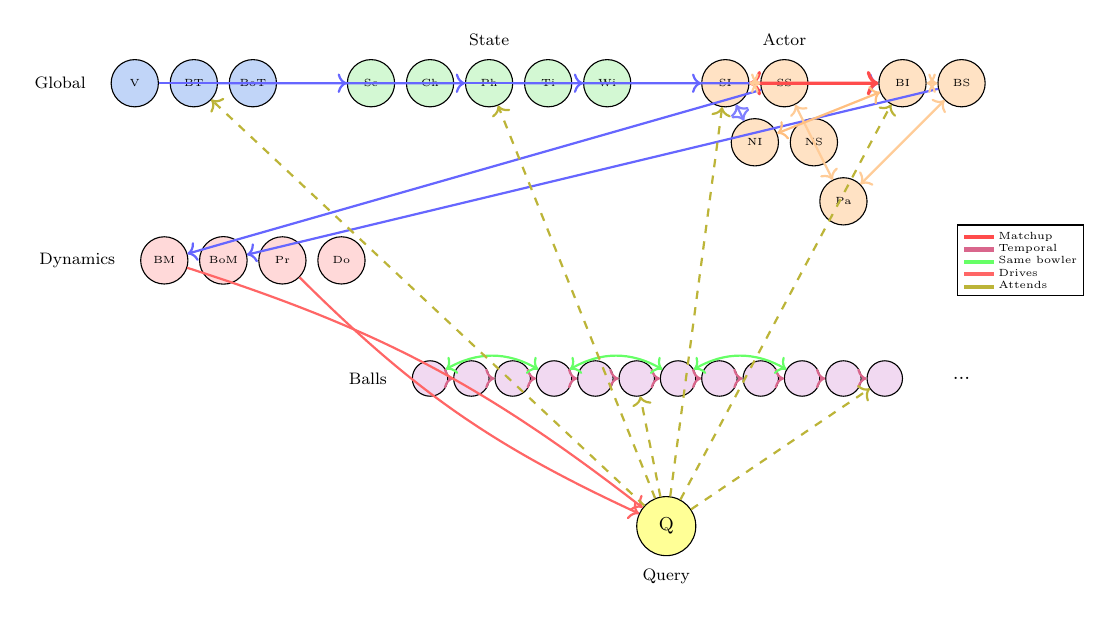
\begin{tikzpicture}[
    gnode/.style={circle, draw, fill=globalcolor!40, minimum size=0.8cm, font=\tiny},
    snode/.style={circle, draw, fill=statecolor!40, minimum size=0.8cm, font=\tiny},
    anode/.style={circle, draw, fill=actorcolor!40, minimum size=0.8cm, font=\tiny},
    dnode/.style={circle, draw, fill=dynamicscolor!40, minimum size=0.8cm, font=\tiny},
    bnode/.style={circle, draw, fill=ballcolor!40, minimum size=0.6cm, font=\tiny},
    qnode/.style={circle, draw, fill=querycolor, minimum size=1cm, font=\small},
    edge/.style={->, gray, thick},
    biedge/.style={<->, gray, thick},
    scale=0.75, transform shape
]
    % Global nodes
    \node[gnode] (g1) at (-6, 6) {V};
    \node[gnode] (g2) at (-5, 6) {BT};
    \node[gnode] (g3) at (-4, 6) {BoT};

    % State nodes
    \node[snode] (s1) at (-2, 6) {Sc};
    \node[snode] (s2) at (-1, 6) {Ch};
    \node[snode] (s3) at (0, 6) {Ph};
    \node[snode] (s4) at (1, 6) {Ti};
    \node[snode] (s5) at (2, 6) {Wi};

    % Actor nodes (now 7 with non-striker)
    \node[anode] (a1) at (4, 6) {SI};
    \node[anode] (a2) at (5, 6) {SS};
    \node[anode] (a6) at (4.5, 5) {NI};
    \node[anode] (a7) at (5.5, 5) {NS};
    \node[anode] (a3) at (7, 6) {BI};
    \node[anode] (a4) at (8, 6) {BS};
    \node[anode] (a5) at (6, 4) {Pa};

    % Dynamics nodes
    \node[dnode] (d1) at (-5.5, 3) {BM};
    \node[dnode] (d2) at (-4.5, 3) {BoM};
    \node[dnode] (d3) at (-3.5, 3) {Pr};
    \node[dnode] (d4) at (-2.5, 3) {Do};

    % Ball nodes (sequence)
    \foreach \i in {0,...,11} {
        \node[bnode] (b\i) at (\i*0.7 - 1, 1) {};
    }
    \node at (8, 1) {...};

    % Query node
    \node[qnode] (q) at (3, -1.5) {Q};

    % === EDGES ===

    % Hierarchical: global -> state
    \draw[edge, blue!60] (g1) -- (s1);
    \draw[edge, blue!60] (g2) -- (s3);
    \draw[edge, blue!60] (g3) -- (s5);

    % Hierarchical: state -> actor
    \draw[edge, blue!60] (s1) -- (a1);
    \draw[edge, blue!60] (s3) -- (a3);

    % Hierarchical: actor -> dynamics
    \draw[edge, blue!60] (a2) -- (d1);
    \draw[edge, blue!60] (a4) -- (d2);

    % Actor matchup
    \draw[biedge, red!70, very thick] (a1) -- (a3);
    \draw[biedge, actorcolor!70] (a1) -- (a2);
    \draw[biedge, actorcolor!70] (a3) -- (a4);
    \draw[biedge, actorcolor!70] (a2) -- (a5);
    \draw[biedge, actorcolor!70] (a4) -- (a5);
    \draw[biedge, blue!50] (a1) -- (a6);
    \draw[biedge, orange!50] (a6) -- (a3);

    % Temporal: precedes
    \foreach \i in {0,...,10} {
        \pgfmathtruncatemacro{\j}{\i+1}
        \draw[edge, purple!60] (b\i) -- (b\j);
    }

    % Same bowler (example: balls 0, 3, 6, 9)
    \draw[biedge, green!60, bend left=30] (b0) to (b3);
    \draw[biedge, green!60, bend left=30] (b3) to (b6);
    \draw[biedge, green!60, bend left=30] (b6) to (b9);

    % Dynamics drives query
    \draw[edge, red!60, thick] (d1) to[bend left=10] (q);
    \draw[edge, red!60, thick] (d3) to[bend right=10] (q);

    % Query attends to everything
    \draw[edge, yellow!70!black, dashed] (q) -- (g2);
    \draw[edge, yellow!70!black, dashed] (q) -- (s3);
    \draw[edge, yellow!70!black, dashed] (q) -- (a1);
    \draw[edge, yellow!70!black, dashed] (q) -- (a3);
    \draw[edge, yellow!70!black, dashed] (q) -- (b5);
    \draw[edge, yellow!70!black, dashed] (q) -- (b11);

    % Labels
    \node[left=0.3cm of g1, font=\footnotesize] {Global};
    \node[above=0.1cm of s3, font=\footnotesize] {State};
    \node[above=0.1cm of a2, font=\footnotesize] {Actor};
    \node[left=0.3cm of d1, font=\footnotesize] {Dynamics};
    \node[left=0.3cm of b0, font=\footnotesize] {Balls};
    \node[below=0.1cm of q, font=\footnotesize] {Query};

    % Legend
    \node[draw, fill=white, align=left, font=\tiny] at (9, 3) {
        \textcolor{red!70}{\rule{0.5cm}{2pt}} Matchup\\
        \textcolor{purple!60}{\rule{0.5cm}{2pt}} Temporal\\
        \textcolor{green!60}{\rule{0.5cm}{2pt}} Same bowler\\
        \textcolor{red!60}{\rule{0.5cm}{2pt}} Drives\\
        \textcolor{yellow!70!black}{\rule{0.5cm}{2pt}} Attends
    };
\end{tikzpicture}
\caption{Complete unified graph structure}
\end{figure}

\newpage
%==========================================
\section{Model Architecture}
%==========================================

\subsection{Three-Stage Pipeline}

\begin{figure}[H]
\centering
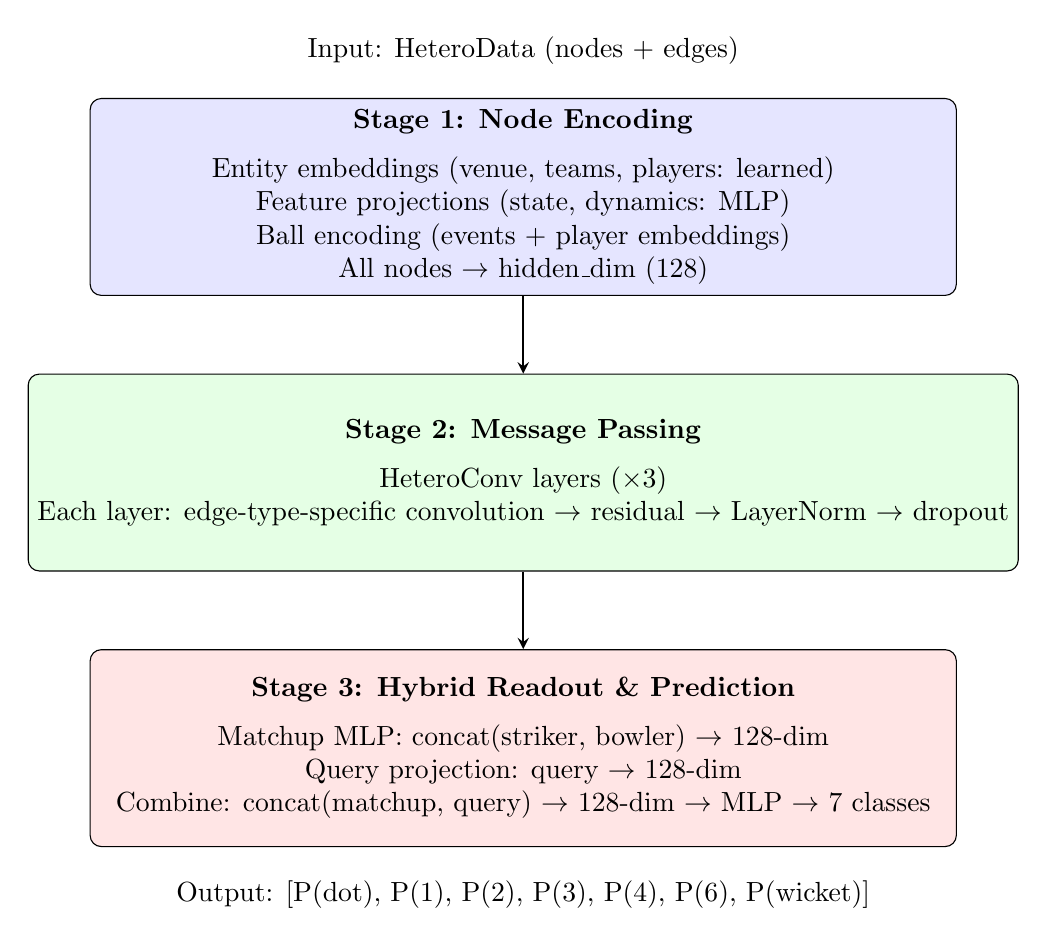
\begin{tikzpicture}[
    stage/.style={rectangle, draw, rounded corners, minimum width=11cm, minimum height=2.5cm, align=center},
    arrow/.style={->, thick, >=stealth}
]
    % Stage 1
    \node[stage, fill=blue!10] (s1) at (0, 6) {
        \textbf{Stage 1: Node Encoding}\\[0.2cm]
        Entity embeddings (venue, teams, players: learned)\\
        Feature projections (state, dynamics: MLP)\\
        Ball encoding (events + player embeddings)\\
        All nodes $\to$ hidden\_dim (128)
    };

    % Stage 2
    \node[stage, fill=green!10] (s2) at (0, 2.5) {
        \textbf{Stage 2: Message Passing}\\[0.2cm]
        HeteroConv layers ($\times$3)\\
        Each layer: edge-type-specific convolution $\to$ residual $\to$ LayerNorm $\to$ dropout
    };

    % Stage 3
    \node[stage, fill=red!10] (s3) at (0, -1) {
        \textbf{Stage 3: Hybrid Readout \& Prediction}\\[0.2cm]
        Matchup MLP: concat(striker, bowler) $\to$ 128-dim\\
        Query projection: query $\to$ 128-dim\\
        Combine: concat(matchup, query) $\to$ 128-dim $\to$ MLP $\to$ 7 classes
    };

    \draw[arrow] (s1) -- (s2);
    \draw[arrow] (s2) -- (s3);

    % Input/Output
    \node[above=0.3cm of s1] {Input: HeteroData (nodes + edges)};
    \node[below=0.3cm of s3] {Output: [P(dot), P(1), P(2), P(3), P(4), P(6), P(wicket)]};
\end{tikzpicture}
\caption{Three-stage model pipeline with hybrid readout}
\end{figure}

\subsection{Hybrid Readout: Why?}

Cricket ball prediction is fundamentally an \textbf{edge-level task}: the outcome depends on the specific striker-bowler matchup, modulated by context.

The hybrid readout combines:
\begin{enumerate}
    \item \textbf{Matchup interaction:} Direct combination of striker and bowler representations after message passing
    \item \textbf{Query aggregation:} Global context (venue, phase, momentum) aggregated by the query node
\end{enumerate}

This respects the geometric structure: prediction is at the matchup level, influenced by graph-level context.

\subsection{Convolution Choices per Edge Type}

\begin{table}[H]
\centering
\begin{tabular}{llp{4.5cm}}
\toprule
Edge Type & Convolution & Rationale \\
\midrule
Hierarchical (conditions) & GATv2Conv & Learn which context matters \\
Intra-layer (relates\_to) & GATv2Conv & Self-attention for interactions \\
Actor matchup & GATv2Conv & Learn matchup dynamics \\
recent/medium\_precedes & TransformerConv & Edge features for temporal distance \\
distant\_precedes & SAGEConv & Simple mean for sparse history \\
same\_bowler/batsman & GATv2Conv & Aggregate spell patterns \\
same\_matchup (causal) & GATv2Conv & Historical matchup outcomes \\
Cross-domain (faced/bowled/partnered) & GATv2Conv & Attention-weighted recency \\
Dynamics (informs) & SAGEConv & Simple aggregation \\
Dynamics (drives) & GATv2Conv & Weight momentum vs pressure \\
Query (attends) & GATv2Conv & Learn what matters for prediction \\
\bottomrule
\end{tabular}
\caption{Edge-type-specific convolution operators}
\end{table}

\newpage
%==========================================
\section{Training: Focal Loss for Class Imbalance}
%==========================================

Cricket outcomes are heavily imbalanced:
\begin{itemize}
    \item Dots: $\sim$35-40\%
    \item Singles: $\sim$25-30\%
    \item Twos: $\sim$5-8\%
    \item Threes: $\sim$1-2\%
    \item Fours: $\sim$12-15\%
    \item Sixes: $\sim$5-8\%
    \item Wickets: $\sim$5\%
\end{itemize}

Standard cross-entropy loss is dominated by the majority class (dots). We use \textbf{Focal Loss}:

\[
\mathcal{L}_{focal} = -\alpha_t (1 - p_t)^\gamma \log(p_t)
\]

where:
\begin{itemize}
    \item $p_t$ = model's probability for the correct class
    \item $\gamma = 2.0$ = focusing parameter (higher = more focus on hard examples)
    \item $\alpha_t$ = optional class weights
\end{itemize}

\textbf{Key insight:} $(1 - p_t)^\gamma$ down-weights ``easy'' examples where the model is already confident, focusing learning on hard/rare cases like wickets.

\subsection{Training Configuration}

\begin{table}[H]
\centering
\begin{tabular}{lc}
\toprule
Parameter & Value \\
\midrule
Hidden dimension & 128 \\
Number of layers & 3 \\
Attention heads & 4 \\
Dropout & 0.1 \\
\midrule
Loss & Focal Loss ($\gamma=2.0$) \\
Optimizer & AdamW (lr=1e-3, wd=0.01) \\
Scheduler & Cosine annealing \\
Early stopping & Patience 10 epochs \\
\midrule
Estimated parameters & $\sim$720K \\
\bottomrule
\end{tabular}
\caption{Model and training configuration}
\end{table}

\newpage
%==========================================
\section{Why Full History Now Works}
%==========================================

\subsection{The Quadratic Problem (V1)}

In V1's Transformer, every ball attends to every other ball:

\[
\text{Attention pairs} = \frac{n(n-1)}{2} = O(n^2)
\]

\begin{table}[H]
\centering
\begin{tabular}{lc}
\toprule
History Length & Attention Pairs \\
\midrule
24 balls & 276 \\
60 balls & 1,770 \\
120 balls (full innings) & 7,140 \\
\bottomrule
\end{tabular}
\caption{Quadratic growth in V1}
\end{table}

\subsection{The Sparse Solution (V2)}

In V2, attention only flows along explicit edges. Cricket structure provides natural sparsity:
\begin{itemize}
    \item Only $\sim$6 bowlers per innings $\to$ sparse same\_bowler
    \item Only $\sim$4-6 batsmen $\to$ sparse same\_batsman
    \item Matchups are intersection of above $\to$ very sparse
    \item Multi-scale temporal limits long-range connections
\end{itemize}

\begin{table}[H]
\centering
\begin{tabular}{lccc}
\toprule
History Length & V1 Attention & V2 Edges & Speedup \\
\midrule
24 balls & 576 & $\sim$150 & 4x \\
60 balls & 3,600 & $\sim$800 & 4.5x \\
120 balls (full innings) & 14,400 & $\sim$2,500 & \textbf{6x} \\
\bottomrule
\end{tabular}
\caption{Computational comparison: V1 vs V2}
\end{table}

\textbf{Key insight:} V2 is not just faster---it's more informative. The 20 context nodes (venue, players, dynamics) provide rich structure that V1 processed separately.

\newpage
%==========================================
\section{Interpretability Benefits}
%==========================================

The unified graph provides natural interpretability:

\begin{enumerate}
    \item \textbf{Edge attention weights}: Which historical balls mattered most?
    \item \textbf{Same-bowler attention}: How much did the bowler's spell inform the prediction?
    \item \textbf{Matchup attention}: How important was the striker-bowler confrontation?
    \item \textbf{Dynamics drives attention}: Was momentum or pressure more influential?
    \item \textbf{Hierarchical attention}: Did venue or match state dominate?
\end{enumerate}

All of these are directly extractable from the GATv2Conv attention weights.

%==========================================
\section{Summary}
%==========================================

The V2 architecture represents cricket prediction as a heterogeneous graph where:

\begin{itemize}
    \item \textbf{21 context nodes} capture venue, teams, match state, players, and dynamics
    \item \textbf{N ball nodes} capture full innings history
    \item \textbf{19 edge types} encode cricket-specific relationships
    \item \textbf{Multi-scale temporal edges} capture patterns at different time scales
    \item \textbf{Causal same\_matchup edges} prevent train-test distribution shift
    \item \textbf{Hybrid readout} combines matchup interaction with global context
    \item \textbf{Focal loss} handles class imbalance
\end{itemize}

This design follows Geometric Deep Learning principles: the inductive bias matches cricket's inherent structure, enabling efficient processing of full innings while respecting symmetries (player attribution, temporal causality).

\end{document}
